% !TeX program = pdflatex
\documentclass[border=6pt]{standalone}
\usepackage{tikz}
\usetikzlibrary{arrows.meta, positioning, calc, fit, backgrounds}

\definecolor{MediumRed}{rgb}{0.925, 0.345, 0.345}
\definecolor{MediumGreen}{rgb}{0.37, 0.7, 0.66}
\definecolor{MediumBlue}{rgb}{0.015, 0.315, 0.45}
\definecolor{DarkBlue}{rgb}{0.05, 0.15, 0.35}

\begin{document}
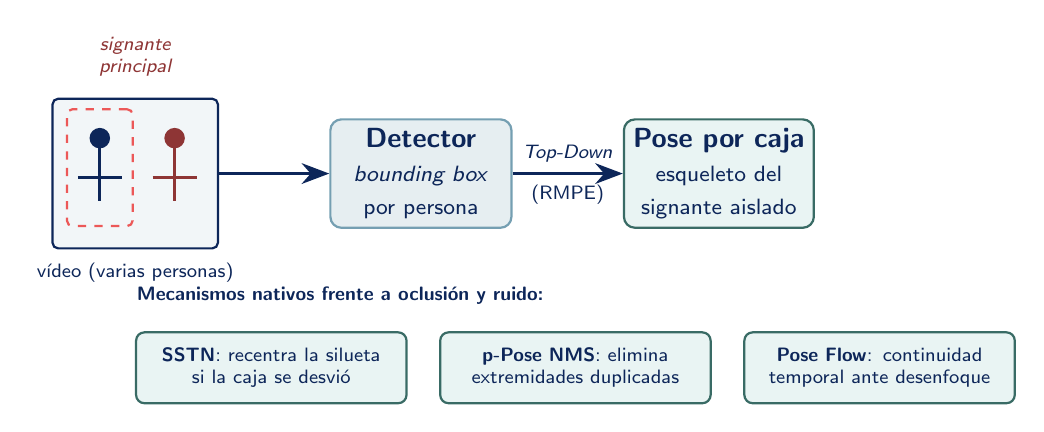
\begin{tikzpicture}[
    font=\sffamily,
    flow/.style={-{Stealth[length=3.5mm]}, line width=1.3pt, DarkBlue},
    stage/.style={draw=MediumBlue!55, thick, rounded corners=4pt, fill=MediumBlue!10,
        text=DarkBlue, align=center, minimum width=2.3cm, minimum height=1.3cm},
    badge/.style={draw=MediumGreen!60!black, thick, rounded corners=3pt,
        fill=MediumGreen!14, text=DarkBlue, align=center, font=\sffamily\scriptsize,
        text width=3.2cm, minimum height=0.9cm},
]

% --- escena de entrada: dos personas ---
\node[draw=DarkBlue, thick, rounded corners=2pt, fill=MediumBlue!5,
      minimum width=2.1cm, minimum height=1.9cm] (scene) at (0,0) {};
\node[font=\sffamily\scriptsize, text=DarkBlue, below=0.05cm of scene]
    {vídeo (varias personas)};
% dos siluetas simples
\foreach \x/\c in {-0.45/DarkBlue, 0.5/MediumRed!60!black}{
    \fill[\c] ($(scene.center)+(\x,0.45)$) circle (0.13);
    \draw[\c, line width=1.2pt] ($(scene.center)+(\x,0.32)$)--($(scene.center)+(\x,-0.35)$);
    \draw[\c, line width=1.2pt] ($(scene.center)+(\x-0.28,-0.05)$)--($(scene.center)+(\x+0.28,-0.05)$);
}

% --- detector ---
\node[stage, right=1.4cm of scene] (det) {\textbf{Detector}\\\footnotesize \emph{bounding box}\\\footnotesize por persona};

% --- pose por caja ---
\node[stage, right=1.4cm of det, fill=MediumGreen!14, draw=MediumGreen!60!black]
    (pose) {\textbf{Pose por caja}\\\footnotesize esqueleto del\\\footnotesize signante aislado};

\draw[flow] (scene) -- (det);
\draw[flow] (det) -- node[above, font=\sffamily\scriptsize, text=DarkBlue] {\textit{Top-Down}} node[below, font=\sffamily\scriptsize, text=DarkBlue] {(RMPE)} (pose);

% caja resaltando al signante principal
\node[draw=MediumRed, thick, dashed, rounded corners=2pt, fit={($(scene.center)+(-0.75,0.7)$) ($(scene.center)+(-0.15,-0.55)$)}] {};

\node[font=\sffamily\scriptsize\itshape, text=MediumRed!60!black, above=0.15cm of scene, align=center]
    {signante\\ principal};

% --- badges de robustez ---
\node[badge, below=1.3cm of det, xshift=-1.9cm] (b1) {\textbf{SSTN}: recentra la silueta si la caja se desvió};
\node[badge, right=0.4cm of b1] (b2) {\textbf{p-Pose NMS}: elimina extremidades duplicadas};
\node[badge, right=0.4cm of b2] (b3) {\textbf{Pose Flow}: continuidad temporal ante desenfoque};

\node[font=\sffamily\bfseries, text=DarkBlue, left=0.15cm of b1] {};
\node[font=\sffamily\scriptsize\bfseries, text=DarkBlue] at ($(b1.north west)+(-0.1,0.45)$) [anchor=west]
    {Mecanismos nativos frente a oclusión y ruido:};

\end{tikzpicture}
\end{document}
